\documentclass[11pt,twocolumn]{article}

\usepackage[margin=0.65in,top=0.70in,bottom=0.70in]{geometry}
\usepackage{booktabs}
\usepackage{graphicx}
\usepackage{float}
\graphicspath{{../results/figures/}}
\usepackage{enumitem}
\usepackage{microtype}
\usepackage{amsmath}
\usepackage{amssymb}
\usepackage{hyperref}
\usepackage{xcolor}
\usepackage{titlesec}
\usepackage{caption}
\usepackage{parskip}

\setlength{\parskip}{3pt}
\setlength{\parindent}{0pt}
\setlength{\columnsep}{0.25in}

\titlespacing{\section}{0pt}{6pt}{3pt}
\titlespacing{\subsection}{0pt}{4pt}{2pt}

\captionsetup{font=small, labelfont=bf, skip=4pt}

\hypersetup{colorlinks=true, linkcolor=blue, citecolor=blue, urlcolor=blue}

\title{\vspace{-1.2cm}%
  \large\textbf{Are You Smarter than DoRA?}\\[2pt]
  \normalsize Reproducing Weight-Decomposed Low-Rank Adaptation\\
  on Competition Mathematics Benchmarks
}
\author{
  Ryan Ye\quad Boaz Ng\quad Leon Jiao\quad Aadi Singla\\
  \small Cornell University, CS 4782 --- Spring 2026
}
\date{\vspace{-0.4cm}}

\begin{document}
\maketitle
\thispagestyle{empty}

\section{Introduction}

Large language model fine-tuning updates billions of parameters at prohibitive cost. Parameter-Efficient Fine-Tuning (PEFT) methods address this by training a small number of adapter parameters while keeping the base model frozen. \textbf{LoRA} \cite{hu2022lora} adds a low-rank update $\Delta W = BA$ to frozen weight $W_0$ and is the dominant PEFT approach, but still shows a gap vs.\ full fine-tuning.

\textbf{DoRA} \cite{liu2024dora} decomposes $W_0$ into magnitude and direction, applying LoRA only to the direction. The key insight is that full fine-tuning makes \emph{large magnitude changes and small direction changes}, while LoRA can only change direction. Separating the two lets DoRA more closely mimic full fine-tuning behavior at the same parameter budget.

We re-implement DoRA from scratch in PyTorch and evaluate on \emph{competition mathematics}---AMC12 2024/2025 and the MATH benchmark---a domain not studied in the original paper. We introduce a three-mode evaluation protocol that reveals a novel ``knows but can't say'' phenomenon in DoRA.

\section{Chosen Result}

We aim to reproduce the primary result of the DoRA paper: \textbf{DoRA consistently outperforms LoRA at the same rank/parameter budget} (paper Table~2, which reports accuracy across commonsense reasoning and math tasks for LLaMA-7B/13B). A secondary claim is that DoRA at half rank ($r{=}8$) matches full-rank LoRA ($r{=}16$), demonstrating superior parameter efficiency.

We chose this result because it is the paper's central empirical claim and directly tests whether the magnitude--direction decomposition provides a measurable advantage over standard LoRA. Reproducing it on a new domain---competition mathematics (AMC12 2024/2025, 50 multiple-choice problems each; MATH benchmark, 723 free-response problems across 5 difficulty levels)---and at a smaller scale (3B vs.\ the paper's 7B--13B) tests the generality of the finding. Our novel contribution is a three-scoring-mode evaluation protocol that decouples \emph{knowledge} from \emph{generation quality}, enabling finer-grained analysis than simple accuracy.

\section{Methodology}

\subsection{DoRA Algorithm}

DoRA adapts a frozen weight $W_0 \in \mathbb{R}^{d \times k}$ as:
\[
  W' = \mathbf{m} \cdot \frac{W_0 + s \cdot BA}{\|W_0 + s \cdot BA\|_c}
\]
where $B, A$ are low-rank LoRA factors ($r \ll \min(d,k)$); $s{=}\alpha/r$; $\mathbf{m}$ is a trainable per-column magnitude vector initialized to $\|W_0\|_c$; and $\|\cdot\|_c$ is the column-wise $\ell_2$ norm. Only $\mathbf{m}$, $B$, $A$ are trained; $W_0$ is frozen.

A critical implementation detail is the \textbf{detach trick} (Eq.~11 in \cite{liu2024dora}): the norm denominator is detached before backpropagation, saving 24.4\% memory on LLaMA-7B at $\sim$0.2pp accuracy cost. After training, \texttt{merge()} fuses $W'$ back into the base weight for zero-overhead inference.

\subsection{Implementation \& Setup}

We compare: (1)~\textbf{PEFT-LoRA} (\texttt{use\_dora=False}), (2)~\textbf{DoRA (PEFT)} (\texttt{use\_dora=True}, reference), and (3)~\textbf{Custom DoRA} (our from-scratch implementation). Base model: Qwen2.5-3B (base and instruct variants), with ${\sim}0.71\%$ parameters trainable across \texttt{q/k/v\_proj} and \texttt{up/down\_proj}.

\textbf{Training data:} \texttt{train\_light} (MATH-lighteval \cite{matheval}, $\sim$7.5K rows), \texttt{train\_heavy} (+NuminaMath-CoT \cite{numina}, $\sim$27.5K total), and \texttt{train\_s1k} (1K subset). A 4-stage leakage-prevention pipeline (exact match $\to$ fuzzy Jaccard $\to$ answer cross-check) removed 0 eval problems.

\textbf{Hyperparameters:} SFTTrainer, rank $r{=}8$, $\alpha{=}32$, dropout $0.05$, LR $10^{-4}$ (cosine, 3\% warmup), effective batch size 16, 1--3 epochs.

\subsection{Evaluation Protocol}

Standard greedy accuracy conflates knowledge with generation quality. We introduce three scoring modes for AMC12's multiple-choice format:
\begin{enumerate}[leftmargin=*, noitemsep, topsep=2pt]
  \item \textbf{Logit}: append ``\texttt{\textbackslash nThe answer is (}'' $\to$ single forward pass $\to$ argmax over A--E logits. Pure \emph{knowledge probe}.
  \item \textbf{Two-pass}: generate a full reasoning chain, then re-read answer logits. Tests whether reasoning improves selection.
  \item \textbf{Greedy}: generate full response, parse \texttt{\textbackslash boxed\{\}}. Standard \emph{generation quality} metric.
\end{enumerate}
This lets us ask: does a model \emph{know} the answer (logit) but \emph{fail to say it} (greedy)?

\section{Results \& Analysis}

\subsection{AMC12 2024}

\begin{table}[H]
\centering
\caption{AMC12 2024 accuracy. $\Delta$ = logit $-$ greedy. Best per column \textbf{bold}.}
\label{tab:amc2024}
\small
\setlength{\tabcolsep}{4pt}
\begin{tabular}{lrrrr}
\toprule
Model & Logit & 2-pass & Greedy & $\Delta$ \\
\midrule
Base (3B-base)     & 32\% & ---  & ---  & ---     \\
Base (3B-inst)     & 34\% & ---  & 44\% & $-10$pp \\
\midrule
LoRA light (base)  & 38\% & 24\% & 18\% & $+20$pp \\
LoRA light (inst)  & \textbf{44\%} & 32\% & 10\% & $+34$pp \\
LoRA heavy (base)  & 34\% & 32\% & 36\% & $-2$pp  \\
\midrule
DoRA light (base)  & 38\% & 28\% & 12\% & $+26$pp \\
DoRA light (inst)  & 36\% & 24\% & 8\%  & $+28$pp \\
DoRA heavy (base)  & 32\% & ---  & \textbf{46\%} & $-14$pp \\
DoRA r4 (base)     & \textbf{44\%} & --- & 16\% & $+28$pp \\
\bottomrule
\end{tabular}
\end{table}

\begin{figure}[H]
  \centering
  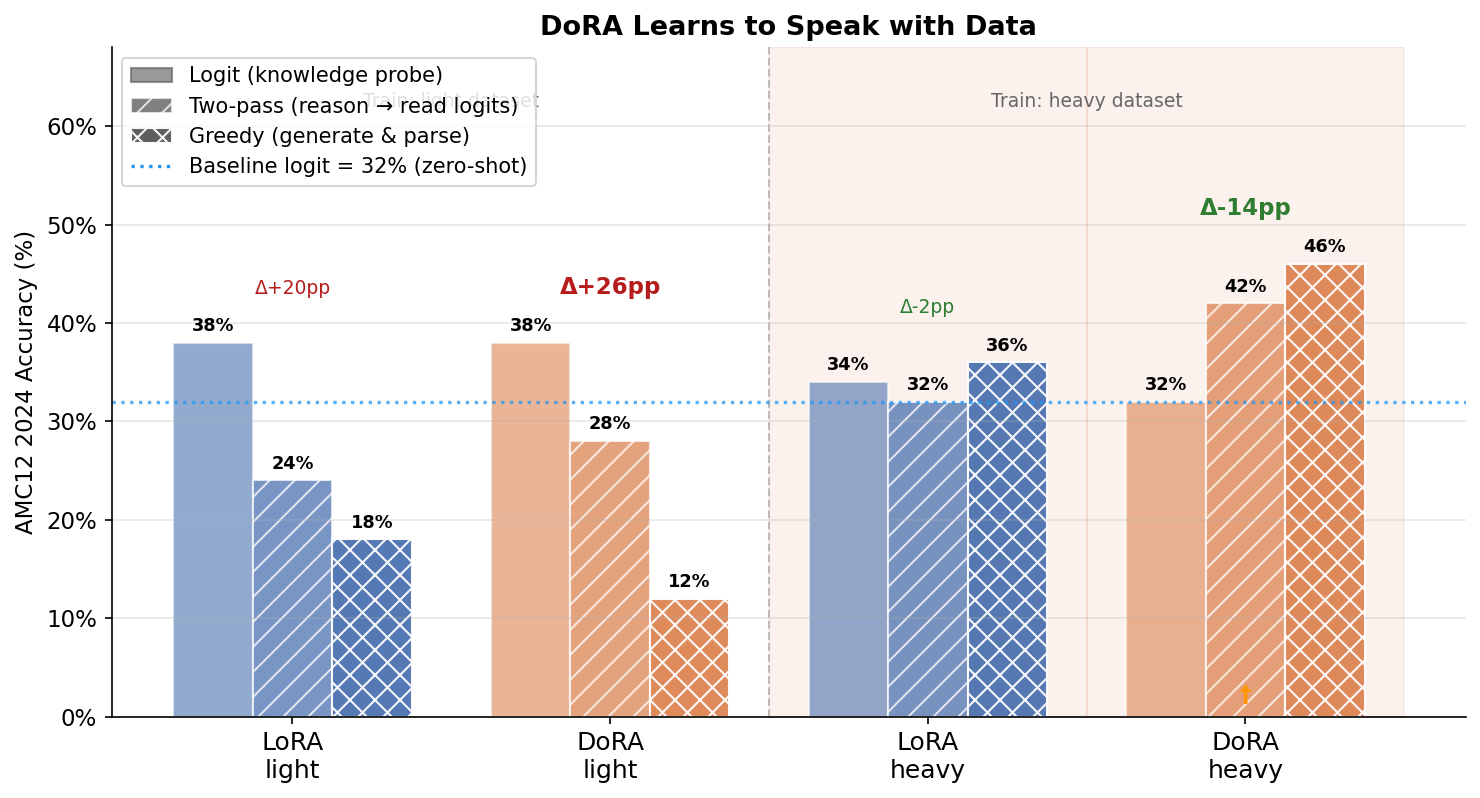
\includegraphics[width=\linewidth]{figI_dora_vs_lora.png}
  \caption{DoRA vs.\ LoRA on AMC12 2024. DoRA's logit--greedy gap is consistently larger. Base model logit (32\%) shown as dotted reference.}
  \label{fig:main}
\end{figure}

\subsection{MATH Benchmark}

\begin{table}[H]
\centering
\caption{MATH benchmark greedy accuracy. Best \textbf{bold}.}
\label{tab:math}
\small
\setlength{\tabcolsep}{4pt}
\begin{tabular}{lrrrr}
\toprule
Model & Overall & L1 & L3 & L5 \\
\midrule
Baseline (base)     & 43.8\% & 74.3\% & 57.6\% & 22.1\% \\
Baseline (inst)     & \textbf{52.7\%} & \textbf{82.6\%} & \textbf{66.1\%} & \textbf{31.4\%} \\
LoRA s1k (inst)     & 44.8\% & 77.1\% & 56.5\% & 24.2\% \\
LoRA heavy (base)   & 35.0\% & 73.4\% & 43.5\% & 15.1\% \\
DoRA light (base)   & 30.7\% & 70.6\% & 36.4\% & 12.7\% \\
\bottomrule
\end{tabular}
\end{table}

\begin{figure}[H]
  \centering
  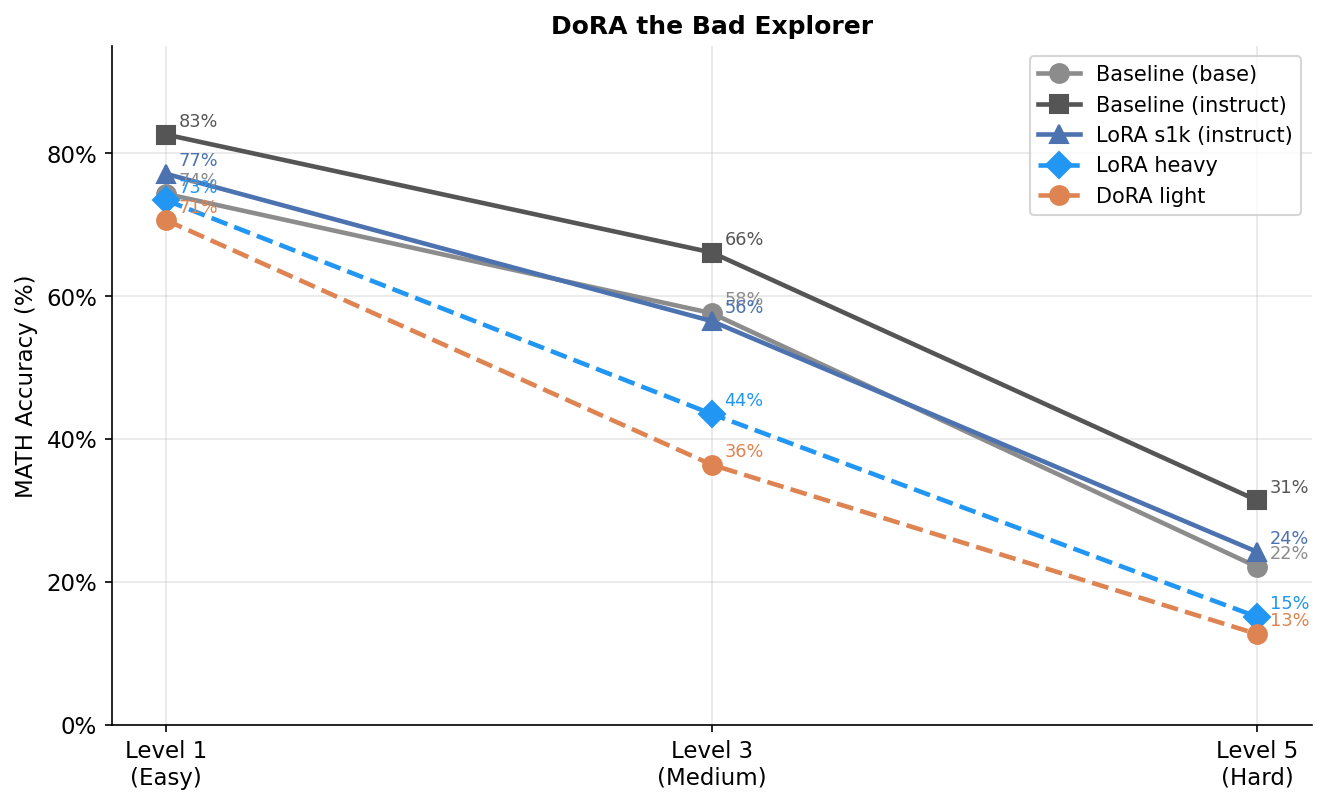
\includegraphics[width=\linewidth]{figG_math_by_level.png}
  \caption{MATH accuracy by difficulty level. DoRA light collapses fastest at hard problems; LoRA s1k tracks the baseline most closely.}
  \label{fig:math}
\end{figure}

\subsection{Key Findings}

\textbf{F1 --- ``DoRA knows but can't say'' (main finding).} DoRA's logit--greedy gap ($\Delta$) is consistently larger than LoRA's at the same configuration: DoRA light $\Delta{=}{+}26$pp vs.\ LoRA light $\Delta{=}{+}20$pp. DoRA assigns high probability to the correct answer internally but fails to produce it through generation, suggesting its magnitude--direction decomposition reorganizes knowledge representations in ways that impede verbalization.

\textbf{F2 --- More data closes and reverses the gap.} LoRA heavy ($3.7{\times}$ more data) nearly equalizes logit and greedy ($\Delta{=}{-}2$pp). DoRA heavy reverses dramatically---greedy (46\%) exceeds logit (32\%), $\Delta{=}{-}14$pp---achieving the best greedy accuracy of any fine-tuned model. DoRA's larger swing suggests it particularly needs training signal to learn fluent generation.

\textbf{F3 --- Knowledge is rank-invariant for DoRA.} Across r2, r4, r8, DoRA logit accuracy stays near 42--44\%, while greedy remains low (12--16\%) at all ranks. LoRA greedy improves more readily with rank, suggesting the gap is a property of DoRA's adaptation mechanism rather than its capacity.

\textbf{F4 --- MATH regression is worse for DoRA.} Fine-tuning on AMC-style data hurts general math reasoning: DoRA light falls 13pp below baseline (30.7\% vs.\ 43.8\%), while LoRA s1k (1K instruct examples) nearly preserves the baseline (44.8\%). Small, targeted datasets appear to cause less catastrophic interference.

\textbf{F5 --- Partial replication.} At the knowledge level (logit), we reproduce the paper's claim: DoRA r4 matches the best LoRA logit result (both 44\%). Greedy accuracy does not confirm DoRA $>$ LoRA at 3B scale---likely due to model scale (3B vs.\ 7B in paper) and our smaller training set.

\subsection{Constraints and Context}
Re-implementation posed three key challenges: the detach trick (Eq.~11) is described briefly but is critical for memory efficiency---omitting it caused OOM on our GPU budget; compute constraints forced us to use Qwen2.5-3B rather than the paper's 7B/13B LLaMA, complicating direct comparison; and the \texttt{train\_heavy} tier mixes MATH-lighteval and NuminaMath-CoT, so accuracy gains may partly reflect distribution shift rather than scale alone. 

Regarding the paper's central claim that decomposing magnitude and direction better mimics full fine-tuning, our results are mixed. DoRA matches or exceeds LoRA on logit-based metrics (representation), confirming the decomposition encodes knowledge effectively. However, DoRA consistently underperforms LoRA on generation accuracy until given substantially more data, suggesting the decomposition disrupts the model's ability to produce correct outputs even when internal representations are strong. We term this the ``knows but can't say'' gap. Crucially, the original paper's evaluation, greedy accuracy on 7B/13B models, would not surface this failure mode, raising the question of whether DoRA's advantages hold at smaller scales or under tighter data regimes.

\section{Reflections}

\textbf{Logit scoring as a knowledge probe.} Our three-mode evaluation was the most important methodological contribution. Without it, we would have concluded a failed replication---DoRA appears to underperform LoRA on generation. Logit scoring revealed DoRA actually \emph{learns the correct answer}; it just cannot always verbalize it. This raises a new research question: can logit-guided or constrained decoding recover DoRA's latent knowledge?

\textbf{Scale matters.} The original paper evaluates 7B--13B models on large, high-quality datasets. At 3B with $\sim$7.5K training examples, we are in a regime where PEFT methods struggle more. Our results suggest 3B is below the threshold where DoRA's generation advantage over LoRA clearly manifests. DoRA heavy (27.5K examples) is the closest we get, achieving the best greedy accuracy---confirming that data scale is the key lever.

\textbf{Future directions.} (1) Scale to 7B+ to match the paper's regime. (2) Apply logit-guided decoding to recover DoRA's latent knowledge. (3) Probe magnitude vectors ($\mathbf{m}$) mechanistically to understand which layers drive the logit--greedy gap.

\newpage
\onecolumn
{\small
\bibliographystyle{plain}
\begin{thebibliography}{9}

\bibitem{liu2024dora}
S.-Y.\ Liu et al.
\textit{DoRA: Weight-Decomposed Low-Rank Adaptation}.
ICML, 2024.

\bibitem{hu2022lora}
E.\ J.\ Hu et al.
\textit{LoRA: Low-Rank Adaptation of Large Language Models}.
ICLR, 2022.

\bibitem{matheval}
DigitalLearningGmbH.
\textit{MATH-lighteval dataset}.
Hugging Face, 2024.
\url{https://huggingface.co/datasets/DigitalLearningGmbH/MATH-lighteval}

\bibitem{numina}
J.\ Li et al.
\textit{NuminaMath-CoT dataset}.
AI-MO / Hugging Face, 2024.
\url{https://huggingface.co/datasets/AI-MO/NuminaMath-CoT}

\bibitem{peft}
S.\ Mangrulkar et al.
\textit{PEFT: State-of-the-art Parameter-Efficient Fine-Tuning methods}.
Hugging Face, 2022.

\bibitem{qwen}
Qwen Team.
\textit{Qwen2.5: A Party of Foundation Language Models}.
Alibaba Cloud, 2024.

\end{thebibliography}
}

\end{document}
